% Requires: \usepackage{tikz} \usepackage{float} \usetikzlibrary{positioning,arrows.meta}
% Compile with pdflatex (or xelatex/lualatex for direct UTF-8 accents).
\documentclass[tikz,border=10pt]{standalone}
\usepackage[utf8]{inputenc}
\usepackage[T1]{fontenc}
\usepackage{float}
\usetikzlibrary{positioning,arrows.meta}

\definecolor{ocTeal}{HTML}{2C7873}
\definecolor{ocOrange}{HTML}{D97F26}

\tikzset{
  hdrteal/.style={rectangle, draw=black, thick, fill=ocTeal, text=white,
    font=\bfseries\footnotesize, align=center, text width=3.4cm, inner sep=5pt},
  hdrorange/.style={rectangle, draw=black, thick, fill=ocOrange, text=white,
    font=\bfseries\footnotesize, align=center, text width=3.9cm, inner sep=5pt},
  body/.style={rectangle, draw=black, thick, fill=white, text=black,
    font=\footnotesize, align=left, text width=3.4cm, inner sep=5pt},
  bodywide/.style={rectangle, draw=black, thick, fill=white, text=black,
    font=\footnotesize, align=left, text width=3.9cm, inner sep=5pt},
  fk/.style={-{Latex[length=2.2mm]}, thick, ocOrange},
  refk/.style={-{Latex[length=2.2mm]}, thick, ocTeal},
  faillink/.style={-{Latex[length=2.2mm]}, thick, dashed, red},
  reflink/.style={-{Latex[length=2.2mm]}, thick, dashed, gray},
}

\begin{document}
\begin{figure}[H]
\small
\centering
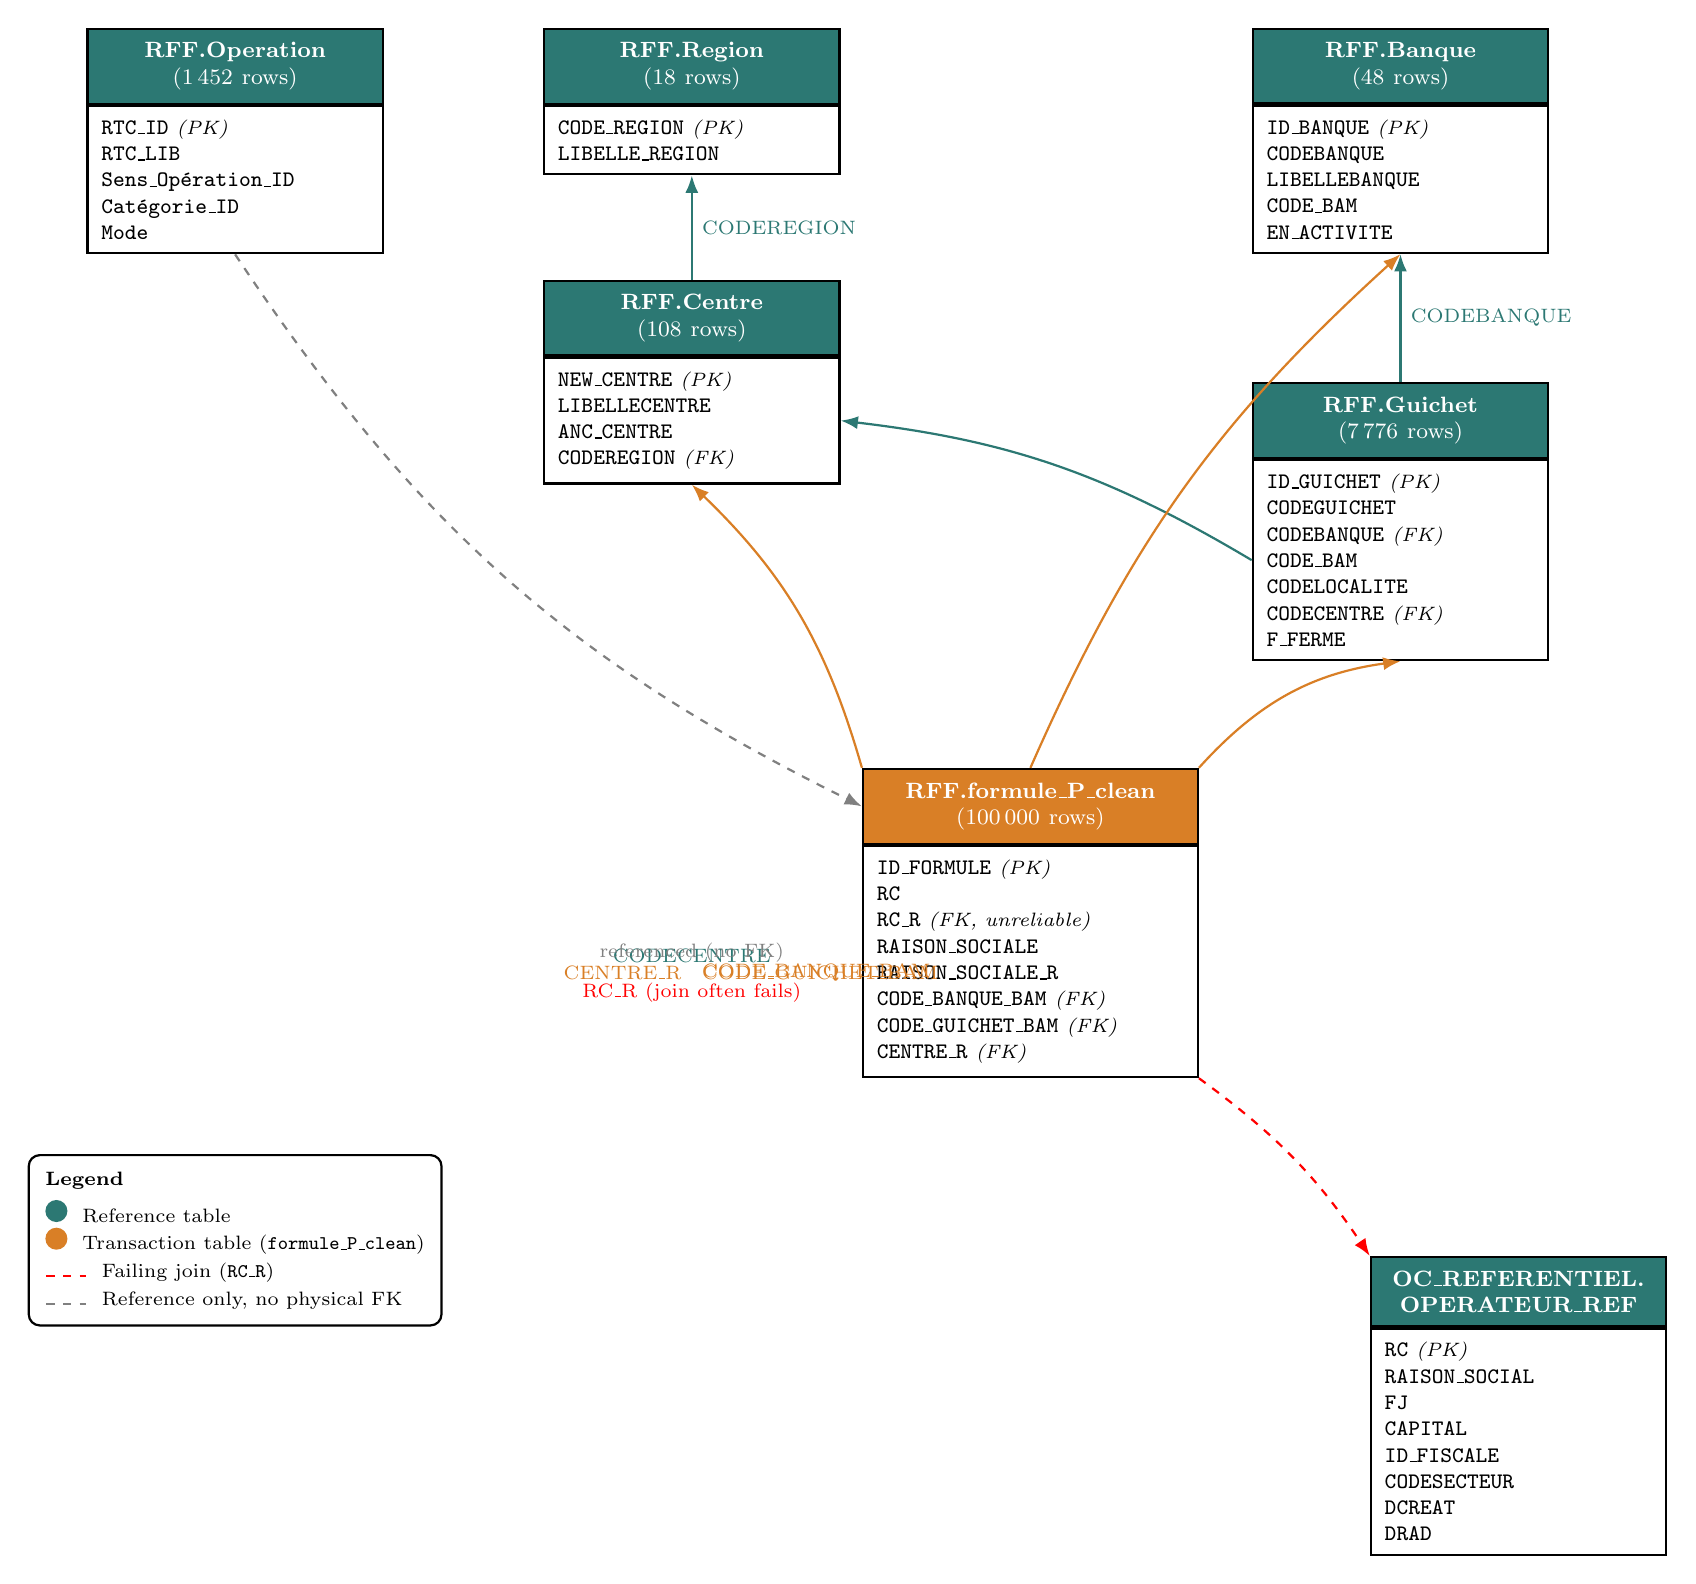
\begin{tikzpicture}[node distance=0pt]

% ---------- RFF.Region ----------
\node[hdrteal, anchor=north] (region-h) at (0,12)
  {RFF.Region \\ \footnotesize\normalfont (18 rows)};
\node[body, below=0pt of region-h] (region-b)
  {\texttt{CODE\_REGION} \textit{\scriptsize(PK)}\\
   \texttt{LIBELLE\_REGION}};

% ---------- RFF.Banque ----------
\node[hdrteal, anchor=north] (banque-h) at (9,12)
  {RFF.Banque \\ \footnotesize\normalfont (48 rows)};
\node[body, below=0pt of banque-h] (banque-b)
  {\texttt{ID\_BANQUE} \textit{\scriptsize(PK)}\\
   \texttt{CODEBANQUE}\\
   \texttt{LIBELLEBANQUE}\\
   \texttt{CODE\_BAM}\\
   \texttt{EN\_ACTIVITE}};

% ---------- RFF.Centre ----------
\node[hdrteal, anchor=north] (centre-h) at (0,8.8)
  {RFF.Centre \\ \footnotesize\normalfont (108 rows)};
\node[body, below=0pt of centre-h] (centre-b)
  {\texttt{NEW\_CENTRE} \textit{\scriptsize(PK)}\\
   \texttt{LIBELLECENTRE}\\
   \texttt{ANC\_CENTRE}\\
   \texttt{CODEREGION} \textit{\scriptsize(FK)}};

% ---------- RFF.Guichet ----------
\node[hdrteal, anchor=north] (guichet-h) at (9,7.5)
  {RFF.Guichet \\ \footnotesize\normalfont (7\,776 rows)};
\node[body, below=0pt of guichet-h] (guichet-b)
  {\texttt{ID\_GUICHET} \textit{\scriptsize(PK)}\\
   \texttt{CODEGUICHET}\\
   \texttt{CODEBANQUE} \textit{\scriptsize(FK)}\\
   \texttt{CODE\_BAM}\\
   \texttt{CODELOCALITE}\\
   \texttt{CODECENTRE} \textit{\scriptsize(FK)}\\
   \texttt{F\_FERME}};

% ---------- RFF.Operation (standalone) ----------
\node[hdrteal, anchor=north] (operation-h) at (-5.8,12)
  {RFF.Operation \\ \footnotesize\normalfont (1\,452 rows)};
\node[body, below=0pt of operation-h] (operation-b)
  {\texttt{RTC\_ID} \textit{\scriptsize(PK)}\\
   \texttt{RTC\_LIB}\\
   \texttt{Sens\_Opération\_ID}\\
   \texttt{Catégorie\_ID}\\
   \texttt{Mode}};

% ---------- RFF.formule_P_clean (central fact table) ----------
\node[hdrorange, anchor=north] (formule-h) at (4.3,2.6)
  {RFF.formule\_P\_clean \\ \footnotesize\normalfont (100\,000 rows)};
\node[bodywide, below=0pt of formule-h] (formule-b)
  {\texttt{ID\_FORMULE} \textit{\scriptsize(PK)}\\
   \texttt{RC}\\
   \texttt{RC\_R} \textit{\scriptsize(FK, unreliable)}\\
   \texttt{RAISON\_SOCIALE}\\
   \texttt{RAISON\_SOCIALE\_R}\\
   \texttt{CODE\_BANQUE\_BAM} \textit{\scriptsize(FK)}\\
   \texttt{CODE\_GUICHET\_BAM} \textit{\scriptsize(FK)}\\
   \texttt{CENTRE\_R} \textit{\scriptsize(FK)}};

% ---------- OC_REFERENTIEL.OPERATEUR_REF ----------
\node[hdrteal, anchor=north] (op-h) at (10.5,-3.6)
  {OC\_REFERENTIEL.\\OPERATEUR\_REF};
\node[body, below=0pt of op-h] (op-b)
  {\texttt{RC} \textit{\scriptsize(PK)}\\
   \texttt{RAISON\_SOCIAL}\\
   \texttt{FJ}\\
   \texttt{CAPITAL}\\
   \texttt{ID\_FISCALE}\\
   \texttt{CODESECTEUR}\\
   \texttt{DCREAT}\\
   \texttt{DRAD}};

% ================= Relationships =================

% Centre -> Region  (Region.CODE_REGION <- Centre.CODEREGION)
\draw[refk] (centre-h.north) -- (region-b.south)
  node[midway, right, font=\scriptsize] {CODEREGION};

% Guichet -> Banque (Banque.CODEBANQUE <- Guichet.CODEBANQUE)
\draw[refk] (guichet-h.north) -- (banque-b.south)
  node[midway, right, font=\scriptsize] {CODEBANQUE};

% Guichet -> Centre (Centre.NEW_CENTRE <- Guichet.CODECENTRE)
\draw[refk] (guichet-b.west) to[bend right=12] (centre-b.east)
  node[midway, above, font=\scriptsize] {CODECENTRE};

% formule_P_clean -> Banque (via CODE_BAM)
\draw[fk] (formule-h.north) to[bend left=12] (banque-b.south)
  node[near end, right, font=\scriptsize, ocOrange] {CODE\_BANQUE\_BAM};

% formule_P_clean -> Guichet (via CODE_BAM)
\draw[fk] (formule-h.north east) to[bend left=20] (guichet-b.south)
  node[near end, right, font=\scriptsize, ocOrange] {CODE\_GUICHET\_BAM};

% formule_P_clean -> Centre (via CENTRE_R)
\draw[fk] (formule-h.north west) to[bend right=15] (centre-b.south)
  node[near start, left, font=\scriptsize, ocOrange] {CENTRE\_R};

% formule_P_clean -> OPERATEUR_REF (RC_R), dashed, failing join
\draw[faillink] (formule-b.south east) to[bend left=10] (op-h.north west)
  node[midway, below, font=\scriptsize, red] {RC\_R (join often fails)};

% Operation: reference-only arrow (no physical FK)
\draw[reflink] (operation-b.south) to[bend right=15] (formule-h.west)
  node[midway, sloped, above, font=\scriptsize, gray] {referenced (no FK)};

% ================= Legend =================
\node[draw, thick, rounded corners, fill=white, align=left, font=\scriptsize,
      inner sep=6pt] (legend) at (-5.8, -3.4) {
  \textbf{Legend}\\[3pt]
  \tikz{\fill[ocTeal] (0,0) rectangle (0.28,0.28);}\ \ Reference table\\[2pt]
  \tikz{\fill[ocOrange] (0,0) rectangle (0.28,0.28);}\ \ Transaction table (\texttt{formule\_P\_clean})\\[2pt]
  \tikz{\draw[red, dashed, thick] (0,0.12) -- (0.5,0.12);}\ \ Failing join (\texttt{RC\_R})\\[2pt]
  \tikz{\draw[gray, dashed, thick] (0,0.12) -- (0.5,0.12);}\ \ Reference only, no physical FK
};

\end{tikzpicture}
\caption{Relational schema of the Office des Changes reference database (RFF / OC\_REFERENTIEL).}
\label{fig:oc-schema}
\end{figure}
\end{document}
